\section{Introduction to Biology} \index{Biology! introduction}

\begin{multicols}{2}


\section*{Characteristics of Living \hfill \\ Things} \index{Living things}


\subsection[Obvious Characteristics of Living Things]{Obvious Characteristics of \hfill \\ Living Things} % Source 10, LASM

\begin{center}
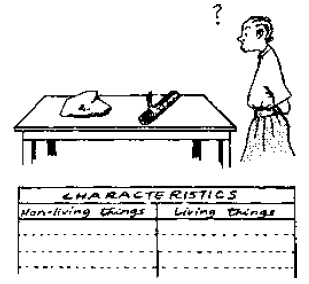
\includegraphics[width=0.45\textwidth]{./img/source/obv-char-living.png}
\end{center}

\begin{description*}
%\item[Subtopic:]{}
%\item[Materials:]{}
%\item[Setup:]{}
\item[Procedure:]{Display some non-living things such as a stone, piece of wood, glass of water etc., and list
any obvious differences between these things and a living organism (i.e. man). Produce a
table from the whole class response.}
%\item[Hazards:]{}
%\item[Questions:]{}
%\item[Observations:]{}
%\item[Theory:]{}
%\item[Applications:]{}
%\item[Notes:]{}
\end{description*}

\subsection{Other Characteristics of Living Things} % Source 11

\begin{center}
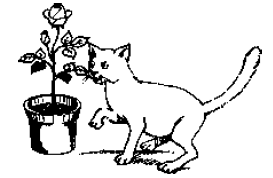
\includegraphics[width=0.4\textwidth]{./img/source/other-char-living.png}
\end{center}

\begin{description*}
%\item[Subtopic:]{}
%\item[Materials:]{}
%\item[Setup:]{}
\item[Procedure:]{Display a potted flowering plant and identify the main characteristics of life. Note that many
of these are less obvious in plants than in animals.}
%\item[Hazards:]{}
%\item[Questions:]{}
%\item[Observations:]{}
%\item[Theory:]{}
%\item[Applications:]{}
%\item[Notes:]{}
\end{description*}

\subsection{Is a Candle Living?} % Source 12

\begin{center}
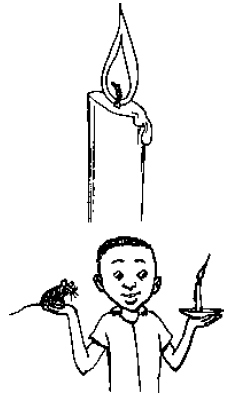
\includegraphics[width=0.4\textwidth]{./img/source/candle-living.png}
\end{center}

\begin{description*}
%\item[Subtopic:]{}
%\item[Materials:]{}
%\item[Setup:]{}
\item[Procedure:]{Look at a burning candle. The candle flame can be considered as an example of a process
in a state of dynamic equilibrium.}
%\item[Hazards:]{}
\item[Questions:]{What are the similarities and differences between a candle flame and a living organism.?}
%\item[Observations:]{}
\item[Theory:]{A candle flame is the result of a metabolic process. The candle wax is burnt to carbon
(soot) and other gaseous substances. The shape, colour and brightness of the flame remains
fairly constant, but only as long as there is a supply of wax and air. The flame is not selfsustained
and cannot reproduce itself.}
%\item[Applications:]{}
%\item[Notes:]{}
\end{description*}

%==================================================================================================%

\section*{Measurement in Biology} \index{Measurement}


\subsection{Data on Height} % Source 17 

\begin{center}
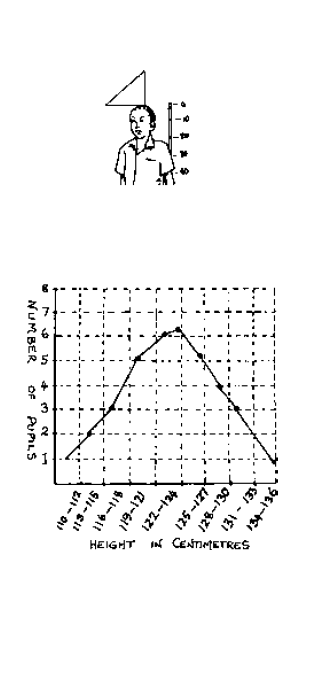
\includegraphics[width=0.45\textwidth]{./img/source/data-height.png}
\end{center}

\begin{description*}
%\item[Subtopic:]{}
%\item[Materials:]{}
%\item[Setup:]{}
\item[Procedure:]{Obtain the heights of all the student in the class (in centimetres). Use these heights to
divide the students into groups (i.e. 110-112 cms, 113-115 cms etc). Count the number of
pupils in each group. Plot a graph of height against numbers.}
%\item[Hazards:]{}
\item[Questions:]{What does the graph look like and what does this show?}
\item[Observations:]{A normal distribution curve is obtained showing that a few students are very tall, a few are
short, but most of them come somewhere between these extremes.}
\item[Theory:]{Members of a species can vary in size between a maximum and a minimum value, but
most individuals are near the middle of this range.}
%\item[Applications:]{}
%\item[Notes:]{}
\end{description*}

\vfill
\columnbreak

\subsection{Data on Pulse Rate} \index{Pulse rate|textbf}

\begin{center}
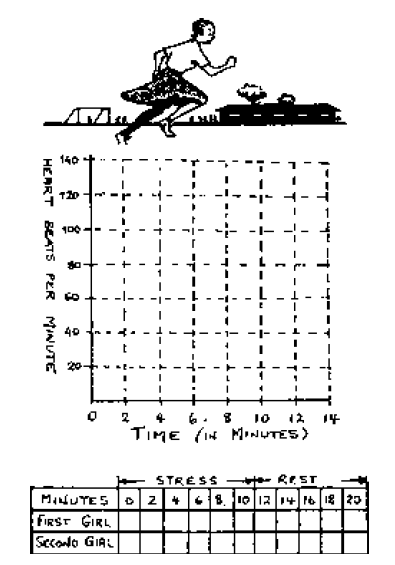
\includegraphics[width=0.4\textwidth]{./img/source/data-pulse.png}
\end{center}

\begin{description*}
%\item[Subtopic:]{}
%\item[Materials:]{}
%\item[Setup:]{}
\item[Procedure:]{Take the resting pulse rate of ten students, then ask them to run around the school
compound for two minutes. Take the pulse of each student at two minute intervals until the
pulse returns to normal. For each student plot a graph of pulse rate against time.}
%\item[Hazards:]{}
\item[Questions:]{Which pulse rate was the highest and which pulse returned to normal most quickly?}
\item[Observations:]{Each curve of pulse rate will be slightly different.}
\item[Theory:]{This is due to differences in levels of physical fitness of each student. The less fit ones
generally reach a higher pulse rate, which takes longer to return to normal.}
%\item[Applications:]{}
%\item[Notes:]{}
\end{description*}

\subsection{Measuring Growth} \index{Growth}

\begin{center}
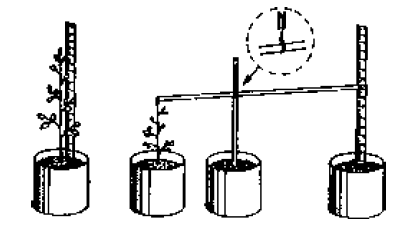
\includegraphics[width=0.4\textwidth]{./img/source/data-growth.png}
\end{center}

\begin{description*}
%\item[Subtopic:]{}
%\item[Materials:]{}
%\item[Setup:]{}
\item[Procedure:]{Take a seedling in a pot (or use a plant in its natural environment) and attach a fine thread
to a light stick (as shown above). Alternatively use the simple method for measuring growth.
Make measurements at fixed intervals (say 2 or 3 days). Devise a method of presenting your
data graphically.}
%\item[Hazards:]{}
%\item[Questions:]{}
%\item[Observations:]{}
%\item[Theory:]{}
%\item[Applications:]{}
%\item[Notes:]{}
\end{description*}

\subsection[Weight Increase by Germinating Seeds]{Weight Increase by \hfill \\ Germinating Seeds} \index{Germination}

\begin{center}
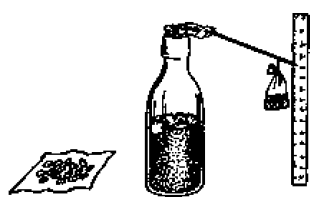
\includegraphics[width=0.45\textwidth]{./img/source/data-weight.png}
\end{center}

\begin{description*}
%\item[Subtopic:]{}
%\item[Materials:]{}
%\item[Setup:]{}
\item[Procedure:]{Place 10 bean seeds between pieces of wet newspaper. Place a second group of 10
beans between dry paper. Measure the weight of each group of beans at daily intervals, and
also record any observations.}
%\item[Hazards:]{}
\item[Questions:]{What are the differences in weight between the two groups of seeds?}
\item[Observations:]{The soaked beans swell and the weight increases. No change occurs in the beans on dry
paper.}
\item[Theory:]{The beans on the wet paper have absorbed water and started germinating. The dry beans
did not.}
%\item[Applications:]{}
%\item[Notes:]{}
\end{description*}

%\columnbreak

\subsection{Keeping a Written Record}

\begin{center}
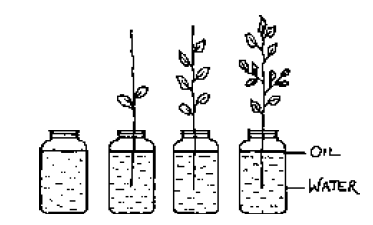
\includegraphics[width=0.45\textwidth]{./img/source/written-record.png}
\end{center}

\begin{description*}
%\item[Subtopic:]{}
%\item[Materials:]{}
%\item[Setup:]{}
\item[Procedure:]{Pick branches with different numbers of leaves and place each one in containers with the
same volume of water (To avoid loss by evaporation pour some oil on the surface). Record
the daily loss of water in each container.}
%\item[Hazards:]{}
%\item[Questions:]{}
\item[Observations:]{The more leaves on the branch, the greater the loss of water.}
\item[Theory:]{Leaves are the organs where most water is lost by the plant.}
%\item[Applications:]{}
%\item[Notes:]{}
\end{description*}

%==================================================================================================%

\section*{The Scientific Method} \index{Scientific method}


\subsection{Transport of Water} \index{Transport} % Source 17 

\begin{center}
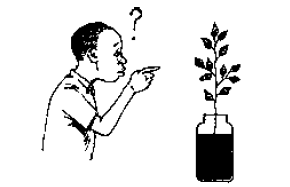
\includegraphics[width=0.45\textwidth]{./img/source/sci-meth-ink-plant.png}
\end{center}

\begin{description*}
%\item[Subtopic:]{}
%\item[Materials:]{}
%\item[Setup:]{}
\item[Hypothesis:]{Water is transported to the leaves where it is lost.}
\item[Procedure:]{Place a branch of a non woody plant in a solution of coloured ink.}
%\item[Hazards:]{}
%\item[Questions:]{}
\item[Observations:]{After some time the coloured ink is seen in the stem and leaves of the plant. A lot of liquid has been absorbed.}
\item[Conclusion:]{The plant transports water upwards through the stem to the leaves where most of
it is lost.}
%\item[Theory:]{}
%\item[Applications:]{}
%\item[Notes:]{}
\end{description*}

\subsection{Number of Leaves and Water Loss}

\begin{center}
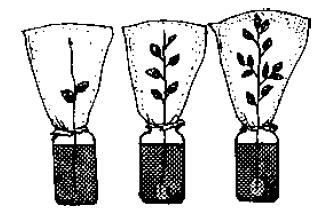
\includegraphics[width=0.4\textwidth]{./img/source/sci-meth-lose-water.png}
\end{center}

\begin{description*}
%\item[Subtopic:]{}
%\item[Materials:]{}
%\item[Setup:]{}
\item[Procedure:]{Using the same materials, place one plastic bag around a single leaf and
another around a branch with many leaves.}
%\item[Hazards:]{}
%\item[Questions:]{}
\item[Observations:]{More water collects in the bag enclosing the larger number of leaves.}
%\item[Theory:]{}
%\item[Notes:]{}
\item[Conclusion:]{Since water is lost from the leaves of a plant, the larger the number of leaves, the
greater the amount of water lost.}
\item[Applications:]{For better growth, plants need to be supplied with an adequate amount of water.
To reduce excessive water losses by transpiration, special methods of cultivation are used.}
%\item[Hypothesis:]{}
\end{description*}

%\subsection{Effect of Sunlight on Plant Growth}
%
%\begin{center}
%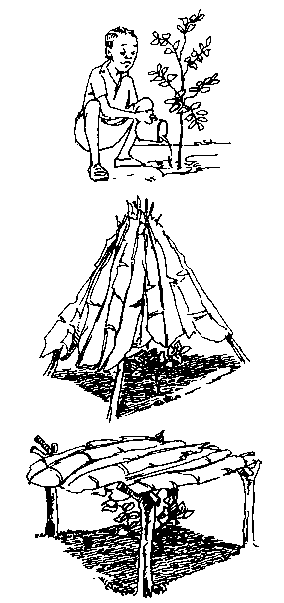
\includegraphics[width=0.4\textwidth]{./img/source/sci-meth-sun-water.png}
%\end{center}
%
%\begin{description*}
%%\item[Subtopic:]{}
%\item[Materials:]{}
%\item[Setup:]{}
%\item[Procedure:]{}
%\item[Hazards:]{}
%\item[Questions:]{}
%\item[Observations:]{}
%\item[Theory:]{}
%\item[Applications:]{}
%\item[Notes:]{}
%\item[Conclusion:]{}
%\item[Hypothesis:]{}
%\end{description*}

\vfill
\pagebreak

%==================================================================================================%



\end{multicols}


\subsection{Hand Washing} \index{Hand washing}

%\begin{center}
%\includegraphics[width=0.4\textwidth]{./img/source/.jpg}
%\end{center}

\begin{description*}
\item[Materials:]{Soap, water, bottle, basin/bucket, chalk, charcoal, food colour, stopwatch}
\item[Setup:]{Prepare a large amount of soapy water. Grind the chalk and charcoal into separate powders.}\\
\item[Problem:]{How long should we wash our hands?\\

\begin{tabular}{|l|c|c|} \hline
\multirow{2}{*}{\textbf{Material}} & \textbf{Hypothesis} & \multirow{2}{*}{\textbf{Experimental Result}} \\
& \textbf{(Seconds)} & \\ \hline
Chalk powder & & \\ \hline
Charcoal powder & & \\ \hline
Food colour & & \\ \hline
\end{tabular} \\[10pt]
}\\
\item[Hypothesis:]{Predict how much time it will take to completely clean your hands and record in the table.}
\item[Procedure:]{Start a stopwatch and have a student or teacher slowly pour soapy water over a basin while the student washes his or her hands. Stop the clock when the student's hands are completely clean.}
\item[Observations:]{Record the time taken to completely wash your hands in the table.}
\item[Questions:]{}\hfill
\begin{enumerate}
\item Why is it important to wash our hands?
\item When do we need to wash our hands?
\end{enumerate}
\item[Theory:]{Washing our hands with soap and water helps to kill harmful bacteria that can cause us to become sick if allowed into our bodies. It is very important to wash our hands before eating and after using the bathroom.}
\end{description*}

\pagebreak


\subsection{Lung Capacity} \index{Lung capacity|textbf}

\begin{center}
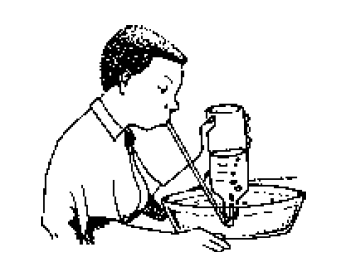
\includegraphics[width=0.4\textwidth]{./img/source/lung-capacity.png}
\end{center}

\begin{description*}
\item[Materials:]{1.5 L bottle, basin, water, plastic tubes/straws, soap, marker, ruler}
\item[Setup:]{Make a scale on the bottle using a marker and ruler (e.g. 100 mL increments). Prepare a soap solution for washing the tubes/straws}\\
\item[Problem:]{How much air can your lungs hold?\\

\begin{tabular}{|l|c|c|} \hline
\multirow{2}{*}{\textbf{Breath}} & \textbf{Hypothesis} & \multirow{2}{*}{\textbf{Experimental Result}} \\
& \textbf{(Volume of air in mL)} & \\ \hline
Normal breath & & \\ \hline
Full breath & & \\ \hline
After holding breath for 10 seconds & & \\ \hline
\end{tabular} \\[10pt]
}
\item[Hypothesis:]{Record the volume of air that you think the lungs can hold for each case in the table.}
\item[Procedure:]{Fill a basin with water. Fill a 1.5 L bottle with water and invert it in the basin so that the mouth of the bottle is underneath the water. Place one end of the tube/straw inside the bottle under water. For each breath, blow into the tube to displace the water.}
\item[Observations:]{Note the reading on the scale before and after blowing into the tube and record the \emph{difference} to give the amount of water displaced.}
\item[Questions:]{}\hfill
\begin{enumerate}
\item Which breath produces the largest amount of air? Which give the smallest amount?
\item How long can you hold your breath?
	\begin{enumerate}
	\item[] Hypothesis: I can hold my breath for \_\_\_\_\_\_\_ seconds.
	\item[] Experimental Result: I can hold my breath for \_\_\_\_\_\_\_ seconds.
	\end{enumerate}
\end{enumerate}
\item[Theory:]{When we breath in air, our bodies use the oxygen and produce carbon dioxide in a process called \emph{respiration}. Oxygen is transported in our blood throughout our bodies. When we hold our breath, oxygen is not circulated throughout our bodies and we begin to feel lightheaded.}
\end{description*}




%\vfill
\pagebreak